\section{Introduction}
Crowdsourcing has emerged as an efficient paradigm for human-solving problem where the requesters ask for certain workers to complete the tasks. Crowdsourcing is introduced by Jeff Howe\cite{howe2006rise} and is it has been applied in various scenarios (data monitoring\cite{DBLP:journals/twc/XuXY15}, language translation\cite{ipeirotis2010analyzing}, image tagging\cite{DBLP:conf/aaai/Tran-ThanhHRRJ15}, mobile crowd sensing\cite{DBLP:conf/cscwd/XuHTXLZ18}, and etc.) to obtain information quickly. Several prominent companies have also developed their crowdsourcing platforms, such as Uber\footnote{Uber is a peer-to-peer ride-sharing, taxi cab, food delivery, bicycle-sharing, and transportation network. Official website is https://www.uber.com/}, DiDi\footnote{DiDi is a Chinese ride-sharing, artificial intelligence (AI) and autonomous technology conglomerate. Official website is https://www.didiglobal.com/}, CTRIP\footnote{CTRIP is a Chinese provider of travel services including accommodation reservation, transportation ticketing, packaged tours and corporate travel management. Official website is https://www.trip.com/}, etc.

The  platforms that we mention have a common feature that the tasks in platform have binding constraint. For example, you and your family have ordered the same tourist route on CTRIP's official website, so you and your family's tourist routes have binding constraint and the platform can't allocate these tourist routes to different travel agencies. For the task assignment problem in crowdsourcing system, there are many works\cite{DBLP:conf/wcnc/CuiS0GDYL18}\cite{liu2018reverse}\cite{DBLP:conf/IEEEcloud/QinZL17} on matching the tasks and the workers. but they doesn't consider that the tasks have binding constraint. It's urgency that using proper approach to solve BTAP. For the platform, binding constraint must be guaranteed, but workers do not necessarily care about binding constraints. In addition to binding constraint, the platform must face with a critical challenges. The worker is selfish and may take self-interested individuals’ strategy to improve own profit. Meanwhile, since the profiles reported by workers will effect their own tasks assignments, the worker may report an untruthful profiles. However, untruthful profiles will do harm on achieving maximum social welfare. Thus, we need to design mechanism by considering the incentives of workers.

In this paper, we consider a simple case that the requester's task just need single skill. In order to ignore requester's task pricing, we adopt the idea of maximum risk and design reserve price for the tasks. After the requester announces a task, the platform will set maximum payment which means that the requester will pay the most price for service. We call maximum payment as reserve price. In our work, we just consider requester has accepted the reserve price and their tasks has existed on the platform. We mainly focus on solving BTAP to achieve minimization of total cost of workers and truthfulness of workers.

Combinatorial auction is good method of achieving truthful mechanism, and has applied to many scenarios (multi-agent pathfinding\cite{DBLP:conf/aaai/AmirSS15}, spectrum sharing\cite{DBLP:conf/icc/ZhanCC15}, decentralized multi-project scheduling\cite{DBLP:conf/atal/SongKZX16}). In corwdsoucing field, Jingmei Cui proposed TCAM\cite{DBLP:conf/wcnc/CuiS0GDYL18} and Haiyan Qin proposed TMC-VCG\cite{DBLP:conf/IEEEcloud/QinZL17}. We adopt their ideas of solving task assignment and use the reverse combinatorial auction to solve the binding task assignment problem (BTAP). We regard the binding tasks as the heterogeneous items, the worker acts as bidder and obtains task by bidding. We formulate the winner determination problem (WDP) a linear programming (LP), and the platform determines winner by solving LP. We use VCG payment rule The way determines the reward of every bidder, use average reward of worker to charge every requester. Especially, we use reserve price to construct a virtual bidder and let virtual bidder participant in solving LP, this way guarantee every requester's payment doesn't exceed reserve price.

In this paper, main contributions are listed as follows. 1) We formulate BTAP as reverse combinatorial auction and propose LP expression of WDP. Especially, we properly address binding constraint of the tasks. 2) We build a virtual worker, which protect payment of requester. 3) we prove our approach achieve nice economic properties, including incentive compatibility, individual rationality and budget balance. The remainder of this paper is structured as follows. We  detailly introduce basic settings about problem in Section 2. Then, we introduce how to solve BTAP by auction model in Section 3. Finally, we evaluate performance of our approach in different setting in Section 4. followed by conclusions in Section 5.

\section{Basic Settings}
In this section, we introduce the basic settings. A typical crowdsourcing system consists of $Q$ requesters and $n$ workers and a platform. In our crowdsourcing system framework, the requester announces tasks through the platform, and the platform assigns the tasks to the workers. The worker will get the reward of from the requester after completing the task, meanwhile, the platform will get the commission on the requester.
\begin{figure}
    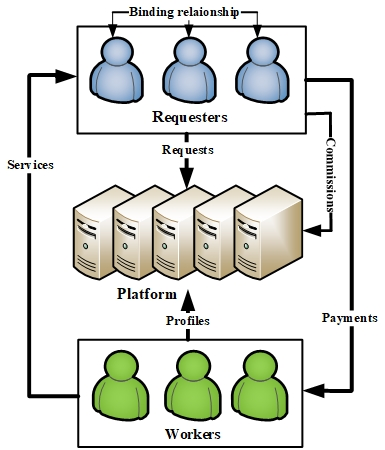
\includegraphics[height=0.45\textwidth, width=0.45\textwidth]{crowdsourcing_system}
    \caption{crowdsourcing system framework with binding tasks}\label{img1}
\end{figure}

Figure \ref{img1} depicts the crowdsourcing system framework with three types of players: multiple requesters and multiple workers, one platform. Next we will introduce these three types of players respectively.

% requester
Here, the requesters want to ask the skillful workers to finish their tasks. we consider a simple case that the requesters just ask for single skill and announce a task. Every requester who has accepted the reserve price $R$ offered by the platform enters the platform and announces a task. Their tasks are homogeneous that we call them as unit tasks. Platform reduces $Q$ unit tasks into $m$ type heterogeneous binding tasks. We use $j \in {1,2,... m}$ represents the index of the binding tasks and use $T_{b} = \{t_1,t_2,\cdots,t_m\}$ denote the set of binding tasks. For each binding task $t_j \in T_{b}$, which we use a tuple $\langle g_j,q_j \rangle$ to describe it. This tuple shows that $t_j$ consists of $g_j$ unit tasks and there are $q_j$ quantity of binding task $t_j$. According to meaning of $q_j$, we can get $\sum_{j=1}^{m} q_j = Q$. Notice that the platform can't divide a binding task $t_j$ into $g_j$ unit tasks to allocate them.

% worker
After reading description of binding tasks, there are $n$ workers who are interested in participating will compete with each other for tasks. We use $i \in \{1,2,... n\}$ represents the index of workers and use $W = \{w_1,w_2,\cdots,w_n\}$ to denote the set of workers, use $n_i$ to denote quantity of unit tasks that $w_i$ want to obtain, we use $d_i$ to denote maximum demand of worker $i$, we can get $n_i \leq d_i$. Each worker $i$ has a cost function $c_i:n_i \rightarrow \mathbb{R} $ which represents the cost of completing $n_i$ unit tasks (With the increase of $n_i$, marginal cost is decreasing), and worker $i$ doesn't know the cost function of others. The cost function of worker is sensitive to $n_i$ and the worker doesn't discriminate between $m$ type binding tasks. Notice that the platform considers how to allocate the binding tasks, while the worker considers how many unit tasks can be obtained. We need to deal properly with differences in their goal.

% profile
In crowdsourcing system, each worker need to report a profile to the platform. The profile of worker can be denoted as tuple $\langle n_i,b_i \rangle$, the profile claims how many unit tasks he/she want to obtain and the cost of finishing these tasks. Notice that the reported cost may not follow the true cost function $c_i$, since the cost of reporting affects the task allocation itself. We should use a truthful mechanism to encourage the workers to report their profiles following to their true cost function. As each worker doesn't know other's information, worker can't sure how many unit task can be obtained. For the format of profiles that worker reports, we need to design suitable format which is able to express their full preferences.

% platform
In crowdsourcing system, a platform should determine binding tasks assignments and reward of the workers and payment of the requesters. Let $a=(a_1,a_2,\cdots,a_n)$ be a allocation of BTAP and $a_i = (a_{i1},a_{i2},\cdots,a_{im})$ is allocation of worker $i$, $a_{ij}$ indicates worker $i$ can obtain how many binding task $j$. A feasible allocation cannot violate binding task supply constraints and worker demand constraints, we use $A$ denote the set of feasible allocations. our goal is minimizing total cost of workers, we can set the optimality criteria on solution $a$ as the minimization of total cost of workers (TCW):
\begin{equation}\label{eq1}
  TCW(a) = \sum_{w_i \in W} c_i\left(N(a_i)\right)
\end{equation}
The function $N(a_i)=\sum_{j=1}^{m}a_{ij}g_j$ maps allocation of binding tasks to quantity of unit tasks. The optimal allocation denote as $a^{\ast} \in argmax_{a \in A} TCW(a)$. The platform should clear the market as much as possible, meanwhile the platform needs to guarantee that the final payment of the requester is not greater than the reserve price (The reason why the requester enters the market is that he/she accepts the reserve price of the platform).

\section{Auction Model}
In this section, we will introduce the single-round and auction-based task allocation model in the crowdsourcing system. We model the interactive procedure between the platform and workers as a reverse combinatorial auction (the platform on behalf of the requesters who accept reserve price organizes the auction). Next, we will introduce the forms of worker bidding, the utility of the workers, the commission of the platform, the average payment of requesters, how to determine winner bids, how to calculate payment of the requesters and reward of the workers, and the theoretical analysis in the end.

In the Section 2, we mention that it's necessary to design a suitable format of bid for the workers to express complex preferences. In our auction model, we adopt XOR bidding language format\cite{Cramton2006Combinatorial} and incorporate cumulative bidding format used in \cite{DBLP:journals/twc/ZhanCLL14}. Every worker $i$ will submit the bids $B_i$ to the platform in format of:
$$B_i = \langle \left(1,b_i(1)\right)\,xor\,\left(2,b_i(2)\right) xor \cdots xor \left(d_i,b_i(d_i)\right)\rangle$$
We define $B$ as the set of bids, and $B_i \in B$. In this format every worker with maximum demand can fully express preference. Notice that we should use an incentive compatibility mechanism to encourage the worker report $b_i$ following $c_i$.

The platform selects a subset of worker $S \subseteq W$ according to the bids that they submit. We define $S$ is the set of winner. Then, the platform allocates $a_i$ to the winning worker $i$, the winning worker $i$ can get $N(a_i)$ unit tasks. After the platform allocates the binding tasks, the platform will calculate reward of the worker $i \in S$. The worker $i$ will get reward $p_i$, and the utility of $w_i$ can be computed as follow:
\begin{equation}\label{eq2}
u_i(a_i)=
\begin{cases}
    p_i - c_i\left(N(a_i)\right)  \, & \text{$ w_i \in S$}\\
    0                             \, & \text{$ w_i \notin S$}
\end{cases}
\end{equation}
After the platform calculate reward of worker $i$, we should compute commission of the platform on the requesters. We use fixed commission rate $\beta$ multiply the difference between reserve prices and the sum of reward of the workers. The commission of the platform can be computed as follow:
\begin{equation}\label{eq3}
  p_p = \beta \cdot \left( R \cdot \sum_{w_i \in S}N(a_i) - \sum_{w_i \in S}{p_i}\right)
\end{equation}
The payment from the requesters is composed of two parts. The first part is the platform's commission, and the second part is the reward of the workers. The calculation formula is as follow:
\begin{equation}\label{eq4}
  p_r = \frac{p_p + \sum_{w_i \in S}{p_i}}{\sum_{w_i \in S}N(a_i)}
\end{equation}

\subsection{Winner Determination and Pricing}
After the platform receives the workers' bidding, the platform should select winner bids according to TCW. In other words, the platform should solve WDP to achieve minimization of TCW. Meanwhile, the platform should guarantee that the payment is not more than reserve price $R$ after the worker completes his/her task, and the market can be cleared as much as possible. We will introduce how to protect the payment of the requesters and how to get the set of winners $S$, how to calculate reward of workers to ensure truthfulness of worker.

In order to guarantee that the average payment of the requesters $p_r$ does not greater than the reserve price $R$, the platform can adopt shill-biding way\cite{Cramton2006Combinatorial} and constructs a virtual worker. Virtual worker regard reserve price $R$ as unit cost, and its maximum demand is $Q$. We use $w_0$ denote virtual worker and it competes with other workers for tasks. Virtual worker will submit the bids in format of:
$$B_0 = \langle(1,R)\,xor\,(2,2\cdot R)xor \cdots xor(Q,Q \cdot R)\rangle$$
We add virtual worker $w_0$ into the set of workers $W$ , we can get new the set of workers $W^{'} = W \, \cup \, \{w_0\}$ and new the new set of bids $B^{'} = B \, \cup \, \{B_0\}$. Because winner selection adopts the lowest bid rule (goal of WDP is minimizing TCW), worker $i$ win $N(a_i)$ unit tasks, the cost of worker $i$ $c_i(N(a_i))$ is not exceed $N(a_i) \cdot R$ and the payment of requesters is not exceed $R$. We will illustrate this point in the theoretical analysis. If the tasks is allocated to virtual worker, the tasks are fail to be allocated.

Now, we formulate WDP as LP that we define it as LP-1. We introduce a new decision variable $y_{ik}$ which a 0–1 integer variable. $y_{ik}$ represents that the worker $i$ obtains $k$ unit tasks if $y_{ik} = 1$, and doesn't obtain $k$ unit tasks otherwise. The objective function of LP-1 is listed as follow:
\begin{equation}\label{eq5}
  min \sum_{i=0}^{n}\sum_{k=1}^{d_i}b_{ik}y_{ik}
\end{equation}
Here, $b_{ik}$ which indicates the reported cost of worker $i$ completing $k$ tasks. Although $b_{ik}$ has same meaning with $b_i(k)$, $b_{ik}$ can construct linear objective expression instead of nonlinear objective expression using $b_i(k)$. We will introduce the constraints of LP-1 next.

1) The supply constraints: The binding tasks $j$ that allocate to the worker can't over the supply.
\begin{equation}\label{eq6}
  \sum_{w_i \in S}a_{ij} \leq q_j,\, \forall t_j \in T_b
\end{equation}
2) The demand constraints: The quantity of unit tasks that allocates to the worker can't exceed the maximum demand.
\begin{equation}\label{eq7}
  N(a_i) \leq d_i,\, \forall w_i \in W^{'}
\end{equation}
3) The XOR biding language constraint: In XOR bidding language, the bids that is submitted by the worker $i$ are mutually exclusive.
\begin{equation}\label{eq8}
  \sum_{k=0}^{d_i}y_{ik} = 1,\, \forall w_i \in W^{'}
\end{equation}
4) The binding constraints: The unit tasks that the worker $i$ obtains isn't composed by splitting the binding tasks, and the binding tasks are indivisible.
\begin{equation}\label{eq9}
  \sum_{k=0}^{d_i}k \cdot y_{ik} = N(a_i),\, \forall w_i \in W^{'}
\end{equation}
In section 2, we mention that the platform considers how to allocate the binding tasks, while the worker considers how many unit tasks can be obtained. the platform has different goal with the worker. we use constraint 4) address the difference of goal. The left side of the Eq.(\ref{eq9}) represents the worker's goal, and the right side of the Eq.(\ref{eq9}) represents a allocation which is determined by platform. When we get the LP-1 expression, then we use SCIPopt\cite{GleixnerEtal2018OO}\cite{DBLP:conf/icms/MaherMPRSS16} to solve it.

We apply VCG payment rule to calculate payment of the workers that be selected by the platform in solving LP-1. The winner paid is equal to the loss of total cost of workers. So we can calculate the reward of worker $i$ as follow:
\begin{equation}\label{eq10}
  p_i = TCW(a_{-i}^{\ast}) - TCW_{-i}(a^{\ast})\, \forall w_i \in W
\end{equation}
Here, we use $a_{-i}^{\ast}$ denote optimal allocation of the workers without worker $i$, and we use $TCW_{-i}$ denote total cost of workers without worker $i$. We can get optimal allocation by solving LP-1. In conclusion, we can get algorithm 1.

\floatname{algorithm}{\textbf{Algorithm}}
\renewcommand{\algorithmicrequire}{\textbf{Input:}}
\renewcommand{\algorithmicensure}{\textbf{Output:}}
\begin{algorithm}
    \caption{\textbf{VCG-based Reverse Combinatorial Auction}}
    \begin{algorithmic}[1]
        \Require $T_b$, $W$, $B$, $R$, $Q$
        \Ensure $S$, $a^{\ast}$, $P$
        \State Use $R$ and $Q$ construct virtual worker $w_0$  and bids $B_0$
        \State Construct the new set $W^{'} = W\,\cup\,\{w_0\}$; $B^{'} = B\,\cup \,\{B_0\}$
        \State Use $B^{'}$ and $W^{'}$ to solve LP-1 get $a^{\ast}$
        \State Initialize winner set $S = \emptyset$ and payment set $P = \emptyset $
        \For{$w_i \in W$}
            \If{$N(a_i^{\ast}) \neq 0$}
                \State $S = S \,\cup\,\{w_i\}$
            \EndIf
        \EndFor
        \For{$w_i \in S$}
            \State Use $W^{'} \setminus \{w_i\}$ and $B^{'} \setminus \{B_i\}$ to solve LP-1 get $a_{-i}^{\ast}$
            \State Calculate $p_i = TCW(a_{-i}^{\ast}) - TCW_{-i}(a^{\ast})$
            \State $P = P \, \cup \,\{p_i\}$
        \EndFor\\
        \Return $S$, $a^{\ast}$ ,$P$
    \end{algorithmic}
\end{algorithm}
\subsection{Theoretical Analysis}
In this section, we prove the three desirable properties of the our auction approach given specification of a reserve
price: truthfulness, individual rationality and budget balance.\\
\textbf{Theorem 1:} The worker is truthfulness in auction.\\
\textbf{Proof:} We assume that worker $i$ is untruthful but other's are truthful. let $\tilde{a^{\ast}}$ is optimal allocation under untruthful biding and we use $a^{\ast}$ represents the optimal allocation under truthful biding. If every worker reports truth cost, objective function of LP-1 is consistent with TCW and solution of LP-1 is optiaml allocation of BTAP. Therefore, $\tilde{a^{\ast}}$ may not be optimal allocation of BTAP, we can get $TCW(\tilde{a^{\ast}}) \geq  TCW(a^{\ast})$. We define the $u_i$ as utility of worker $i$ under truthful bidding, We define the $\tilde{u_i}$ is utility of worker $i$ under untruthful bidding, and worker $i$ will get $\tilde{n_i}$.

Now, we will prove that worker $i$ dominant strategy is truthful bidding under other worker is truthful:
$$
\begin{aligned}
  u_i(n_i) & = p_i - c_i(n_i) \\
        {} & = TCW(a_{-i}^{\ast}) - TCW_{-i}(a^{\ast}) - c_i(n_i)\\
        {} & = TCW(a_{-i}^{\ast}) - TCW(a^{\ast})\\
        {} & \geq TCW(a_{-i}^{\ast}) - TCW(\tilde{a^{\ast}})\\
        {} & = \tilde{u_i}(\tilde{n_i})
\end{aligned}
$$
\textbf{Lemma 1:} Pre unit cost of winning worker in auction is not exceed reserve price $R$.\\
\textbf{Proof:} We consider of two cases. Case 1: $\forall i \, ,k\, , c_{ik} <= k \cdot R$, it is obvious that \textbf{Lemma 1} is true. Case 2: $\forall i , \, \exists k ,\, c_{ik} > k \cdot R$, if $\exists j \neq i ,\, c_{jk} <= k \cdot R$, the platform will allocate $k$ unit tasks to $j$, if $\forall j ,\, c_{jk} > k \cdot R$, the platform will allocate $k$ unit tasks to virtual worker $w_0$. In conclusion, winning worker's pre unit cost is under reserve price $R$.\\
\textbf{Theorem 2:} The requester and the worker are individual rationality.\\
\textbf{Proof:}\\
1) For the requester, we should prove $p_r \leq R$. According to \textbf{Lemma 1}, the reward of worker $i$ winning $n_i$ unit tasks.
$$
\begin{aligned}
p_i(n_i) & = TCW(a_{-i}^{\ast}) - TCW_{-i}(a^{\ast}) \\
{}       & = TCW(a_{-i}^{\ast}) - (TCW(a^{\ast}) - c_i(n_i)))\\
{}       & \leq Q\cdot R - (Q\cdot R - n_i\cdot R)\\
{}       & = n_i \cdot R
\end{aligned}
$$
Therefore, pre unit reward of worker is not exceed $R$. According to Eq.(\ref{eq3}) and Eq.(\ref{eq4}), we can get the average payment of requesters is not exceed $R$.\\
 2) For the worker, we should prove $u_i \geq 0$. In \textbf{Theorem 1}, we mention that $a^{\ast}$ is optimal allocation of BTAP. Therefore, we can get the $TCW(a_{-i}^{\ast}) \geq TCW(a^{\ast})$. Then we can get:
 $$
  \begin{aligned}
    u_i(n_i) & = p_i - c_i(n_i) \\
        {} & = TCW(a_{-i}^{\ast}) - TCW_{-i}(a^{\ast}) - c_i(n_i)\\
        {} & = TCW(a_{-i}^{\ast}) - TCW(a^{\ast})\\
        {} & \geq 0
  \end{aligned}
 $$
\textbf{Theorem 3:} The platform is budget balance.\\
\textbf{Proof:} We should prove that commission of the platform is non-negative. According to \textbf{Theorem 2}, we can get the commission (we use $n_i$ presents the number of unit task which worker $i$ obtain):
$$
\begin{aligned}
  p_p & =    \beta \cdot \left( R \cdot \sum_{w_i \in S}N(a_i) - \sum_{w_i \in S}{p_i}\right) \\
  {}  & \geq \beta \cdot \left( R \cdot \sum_{w_i \in S}N(a_i) - \sum_{w_i \in S} R \cdot N(a_i) \right)\\
  {}  & = 0
\end{aligned}
$$
\section{Experiment}
In this section, we evaluate our auction approach in the crowdsourcing system environment with different simulation settings. Firstly, we should specify the expression form of the cost function of the worker and define some metrics which is used to evaluate the performance. Then, we give simulation setting. Finally, we analyze the performance result under various settings.

In the Section 2, we mention the cost function of worker and marginal cost is decreasing function, but we don't give specific expression of function. In order to build environment of experiment, we specify the expression form of the cost function of the worker. We think that the cost function consist of two part. The first part is variable cost and the second part is fixed cost. We list the expression as below:
\begin{equation}\label{eq11}
  c_i(n_i) = c_i^v + c_i^f = p_s \cdot \theta_v^{\left(-n_i / d_i\right)} + d_i^{\theta_f}
\end{equation}
Here, variable cost $c_i^v$ is equal to $p_s \cdot \theta_v^{(-n_i/d_i)}$, let $p_s$ denote to the worker based unit cost for completing a unit task, we assume the based unit cost is same. Let $\theta_v^{(-n_i / d_i)}$ denote to the decreasing factor of unit cost, we assume that $\theta_v$ is varied among the workers. Fixed cost $c_i^f$ is equal to $d_i^{(\theta_f)}$ , we assume that $\theta_f$ is vary among the workers.

Here, we define some metrics to evaluate our approach. In section 3, we illustrate our approach may not be able to clear market (the tasks may not be completely assigned). We want to explore which settings is better for clearing market. We define the tasks clearing ratio $TCR$ as follow:
\begin{equation}\label{eq12}
  TCR = \frac{\sum_{w_i \in S} N(a_i)}{Q}
\end{equation}
In order to explore the profit of workers. we define the average worker profit ratio $AWPR$ as follow:
\begin{equation}\label{eq13}
  AWPR = \frac{1}{|S|}\sum_{w_i \in S}\frac{u_i}{p_i}
\end{equation}
let $|S|$ represent the number of winner. In section 3, we build a virtual worker protect the requester's offer. In order to characterize the degree of protection for requesters, we define the average requester protection ratio $ARPR$ as follow:
\begin{equation}\label{eq14}
  ARPR = \frac{R - p_r}{R}
\end{equation}
The larger the $ARPR$ is, the better the degree of protection is, and the requester will be more willing to accept the reserve price. According to Eq.(\ref{eq3}). the platform will get more commission with $ARPR$ increasing.
\begin{figure}
  \centering
  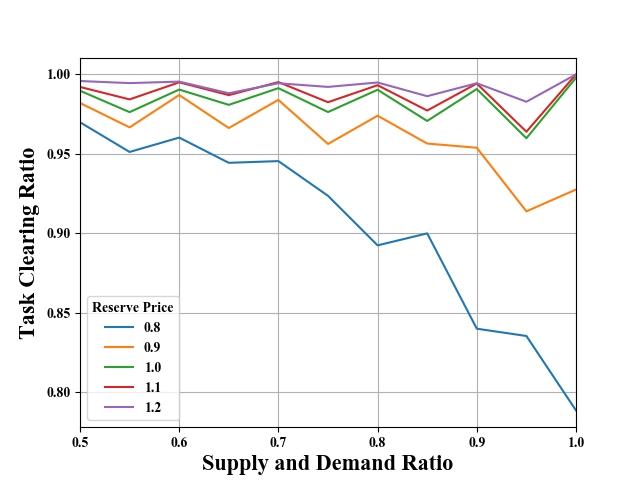
\includegraphics[width=0.6\linewidth]{performance1.png}
  \caption{Performance of Market Clearing}\label{img2}
\end{figure}

\begin{figure}
  \centering
  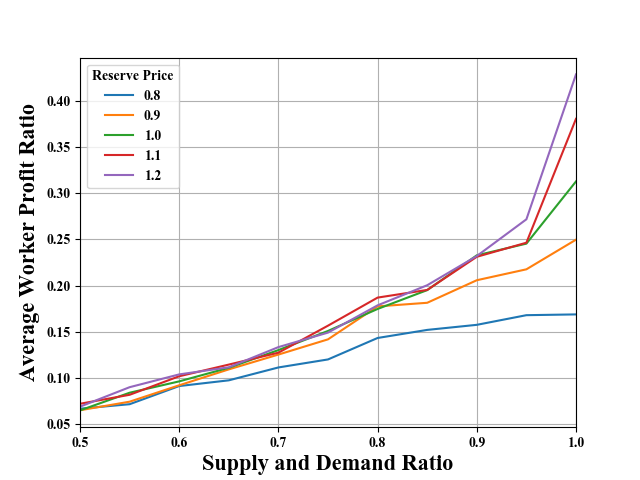
\includegraphics[width=0.6\linewidth]{performance2.png}
  \caption{Performance of Worker's Profit}\label{img3}
\end{figure}

\begin{figure}
  \centering
  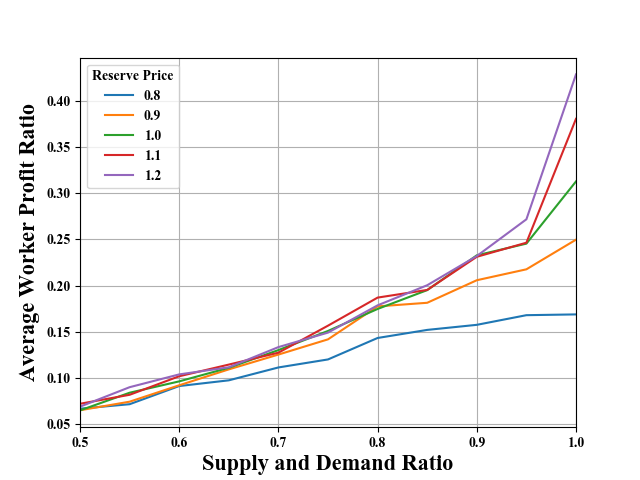
\includegraphics[width=0.6\linewidth]{performance2.png}
  \caption{Performance of Requester's Payment}\label{img4}
\end{figure}
%\begin{figure*}[htbp]
%\centering
%\subfigure[Performance of Market Clearing]{
%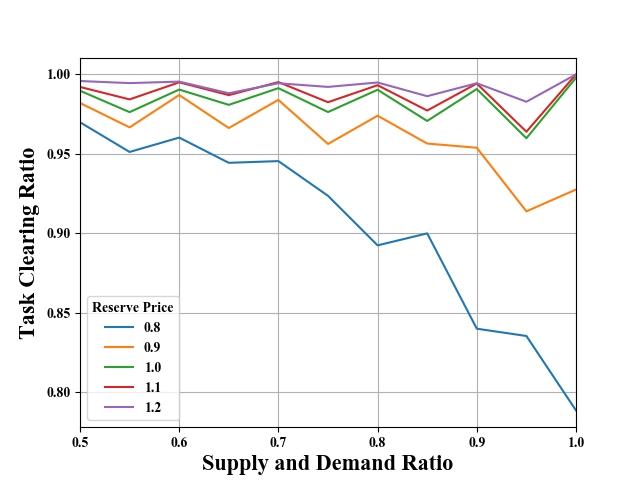
\includegraphics[width=0.3\linewidth]{performance1.png}
%}\label{img2a}
%\subfigure[Performance of Worker's Profit]{
%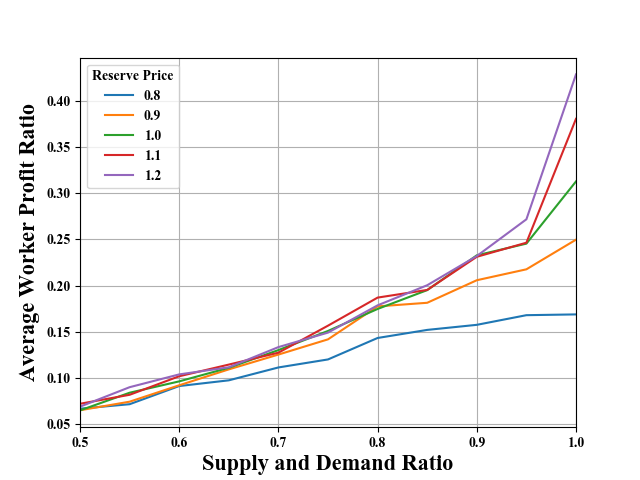
\includegraphics[width=0.3\linewidth]{performance2.png}
%}\label{img2b}
%\subfigure[Performance of Requester's Payment]{
%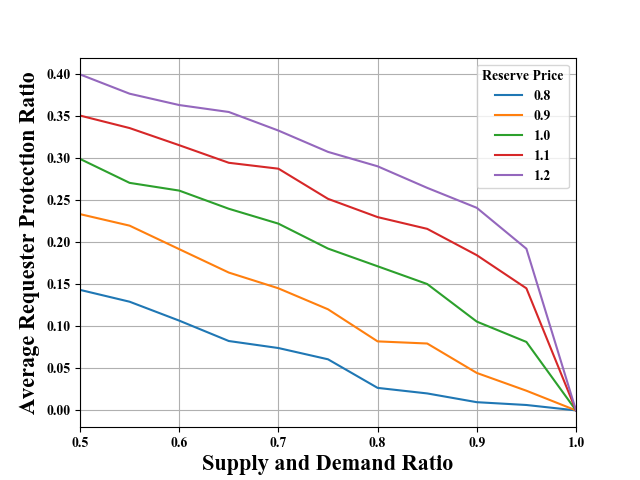
\includegraphics[width=0.3\linewidth]{performance3.png}
%}\label{img2c}
%\centering
%\caption{Performance of Auction Model with Different Settings}\label{img2}
%\end{figure*}
\subsection{simulation setting}
For parameters of cost function we set $\theta_{v} \sim U(1.2,e)$, and $\theta_{f} \sim U(0.3,0.4) $,we sample $d_i$ from $\{10,11,\cdots,29,30\}$, let $p_s$ is equal to $1.0$. For the workers, we fix the number of workers $n$ is 10. For binding task, we define maximum binding task as $t_m = \mathop{\arg\max}_{t_j \in T_b} g_j$, and $t_m$ is sampled from ${1,2,\cdots,5,6}$. For the platform, reserve price $R$ is generated by increments 0.1 between 0.8 to 1.2. Here, we define $\alpha = \frac{Q}{\sum_{w_i \in W} d_i}$ as supply and demand ratio, and $\alpha$ is generated by increments 0.05 between 0.5 to 1.0.

In our experiment, we mainly explore the performance of auction in different of $\alpha$ and $R$ settings. Each indicated data in the figures is the average result of 100 independent instances in each $\alpha$ and $R$ setting.
\subsection{simulation result}
We get the results by simulating our approach in different settings, and now we analyze the results. In Figure \ref{img2}, when the reserve price $R$ is high relatively, the effect of supply-demand ratio $\alpha$ on the $TCR$ is relatively small, and $TCR$ is stable at a relatively high level. When the reserve price is relatively small, the effect of $\alpha$ on $TCR$ is more obvious. In fact, we can find that when $R geq p_s$, the $TCR$ basically fluctuates above 95\%. Therefore, the platform set a larger reserve price for the task is conducive to market clearing.

In Figure \ref{img3}, we find that the average worker profit ratio $AWPR$ increases with the increase of $\alpha$ regardless of the reserve price, which indicates that the weaker competition in the environment, the higher the income of workers. However, when the reserve price was relatively low, the workers' profit tends to stabilize, which may be due to the low $TCR$. While reserve price are relatively high, the profits of workers show a substantial increase. Therefore, the platform set a larger reserve price for the task is also beneficial for workers to make profits.

In Figure \ref{img4}, regardless of the reserve price, the average requester protection ratio $ARPR$ decreases with the increase of $\alpha$, and the ultimate $ARPR$ is equal to 0. In other words, the requester's payment become higher and higher gradually, and finally is equal to reserve price. At the same time, we find that the larger the reserve price, the better the $ARPR$ which be achieved. Therefore, the larger reserve price on the platform can make the requester pay more self-satisfied payment, the platform itself will also benefit from it.
\section{Conclusion}
In this paper, we study how to allocate tasks with binding constraint to achieve minimization of $TCW$. Meanwhile, we consider also truthfulness of worker. We formulate the allocation process as an auction process. We propose a reasonable LP-1 expression for WDP and use VCG payment rule to guarantee workers report truthful profiles. In the process of bidding, XOR language is used to fully express the complex preferences of workers. In solving WDP process, we take into account the individual rationality of requesters and construct virtual bidders to participate in solving LP-1. Finally, we evaluate our approach through experiments, and find that higher reserve price setting is beneficial to all three types players (platform, requester, worker).  